\section{Data Governance \& Privacy Preservation}\label{sec:datagov}

CYBEX-P offers a robust data governance mechanism with granular access control of data. Here, we discuss the `attribute based access control' protocol of CYBEX-P.

\subsection{Data Model and Privacy Parameters}

%\texttt{Events} contain \texttt{attributes} or \texttt{objects}.
CYBEX-P converts any incoming data into a TAHOE \texttt{event}.  Fig. \ref{fig:priv1} shows an \texttt{event} with two \texttt{attributes} -- an \texttt{IP} and a \texttt{file} (filename). Assume, the data owner \texttt{Org 2} wants to share the \texttt{file} with everyone but not the \texttt{IP}.

\begin{figure}[ht]
	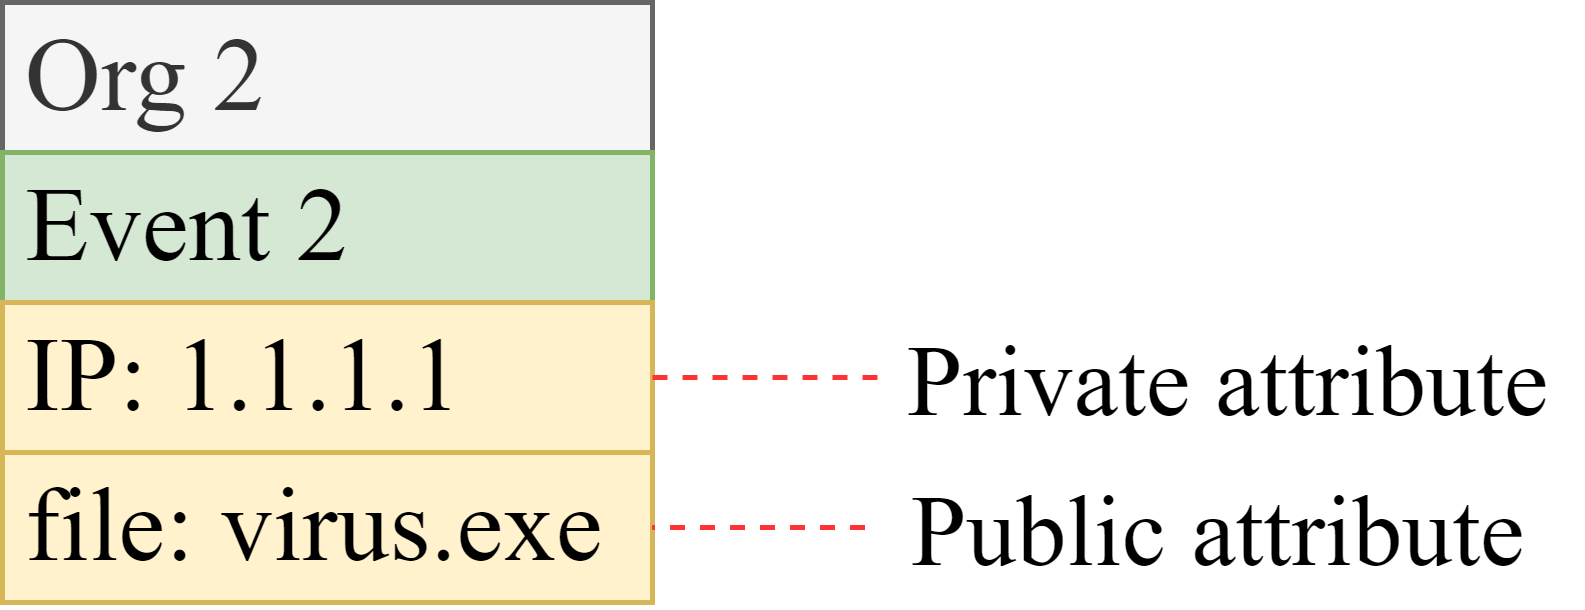
\includegraphics[height=.72in]{data_for_privacy_example} % height = 12*.06
	\centering
	\caption{Data owner determines if an attribute is public or private.}
	\label{fig:priv1}
\end{figure}

%Such a granular control essentially requires attaching an access control list (ACL) to each piece of data. CYBEX-P uses symmetric encryption to achieve such access control. This technique is explained in the following subsections.

\subsection{Public Attribute (Not Encrypted)}

Data owner \texttt{Org 2}, first, converts the document into a TAHOE \texttt{event} as shown in Fig. \ref{fig:priv2}. Here, \texttt{0xABC} is the hash of the IP \texttt{1.1.1.1}, \texttt{0xDEF} is the hash of the file \texttt{virus.exe}, \texttt{0x123} is the hash of the \texttt{event} itself, and acts as the event id. The hashes of the attributes are placed in the \texttt{edge} array creating a graph. Note that, we use the term \texttt{edge} to denote the \texttt{\_ref} array from \ref{ss:graph}.

\begin{figure}[ht]
	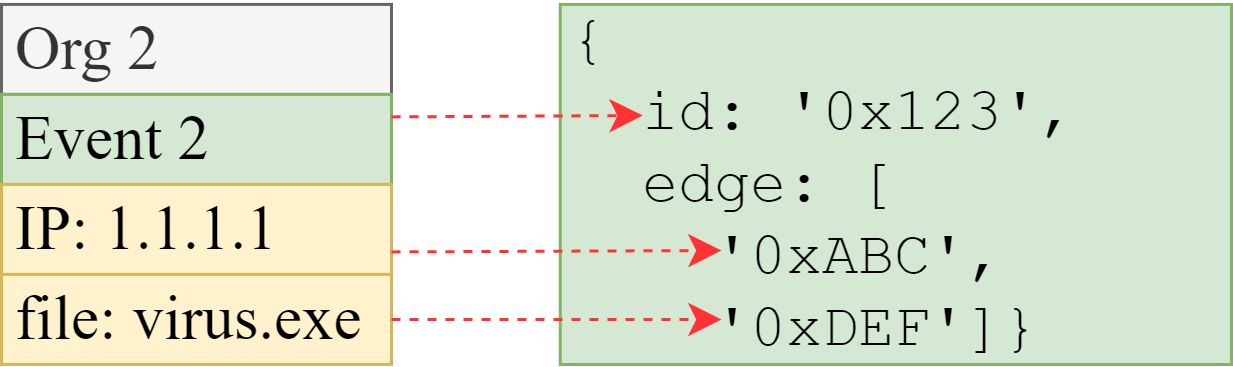
\includegraphics[height=.72in]{data_for_privacy_example_as_tahoe} % height = 12*.06
	\centering
	\caption{Event data in TAHOE format before encryption.}
	\label{fig:priv2}
\end{figure}

%The hash of the event data \texttt{0x123} acts as a globally unique and reproducible id of the data.



\subsubsection*{\textbf{Threat Model}}

The data owner \texttt{Org 2} trusts all participants of CYBEX-P with the public attribute \texttt{virus.exe}.

\subsubsection*{\textbf{Public Data Query}}

\begin{figure}[ht]
	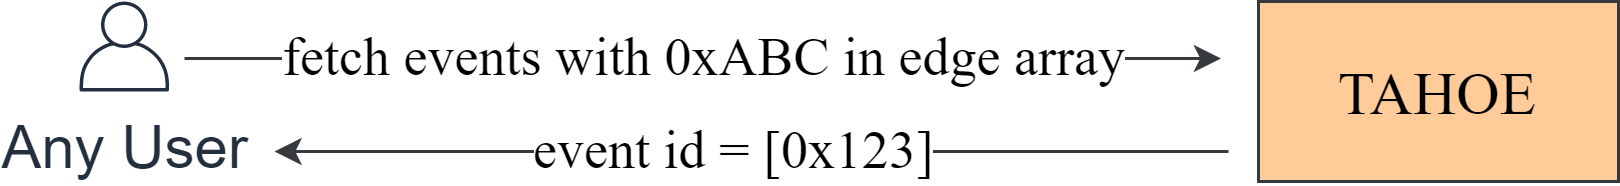
\includegraphics[height=.36in]{public_data_query} %height = 6*.06
	\centering
	\caption{Public Data Query.}
	\label{fig:pubque}
\end{figure}

Now, assume a user wants to get all the events with the file \texttt{virus.exe}. She first generates the hash of \texttt{virus.exe} as \texttt{0xDEF}. Then she looks up the database for events that have \texttt{0xDEF} in the \texttt{edge} array. She will get the \texttt{event 0x123} in return.

\subsection{Private Attribute Encryption}

%AES256  \cite{chown2002advanced}
To protect the private attribute, \texttt{Org 2} encrypts its hash \texttt{0xABC} with \texttt{secret} to generate the ciphertext \texttt{0x789}, as shown in Fig. \ref{fig:priv3}. The owner can use any symmetric encryption technique of choice although TAHOE recommends AES256.

\begin{figure}[ht]
	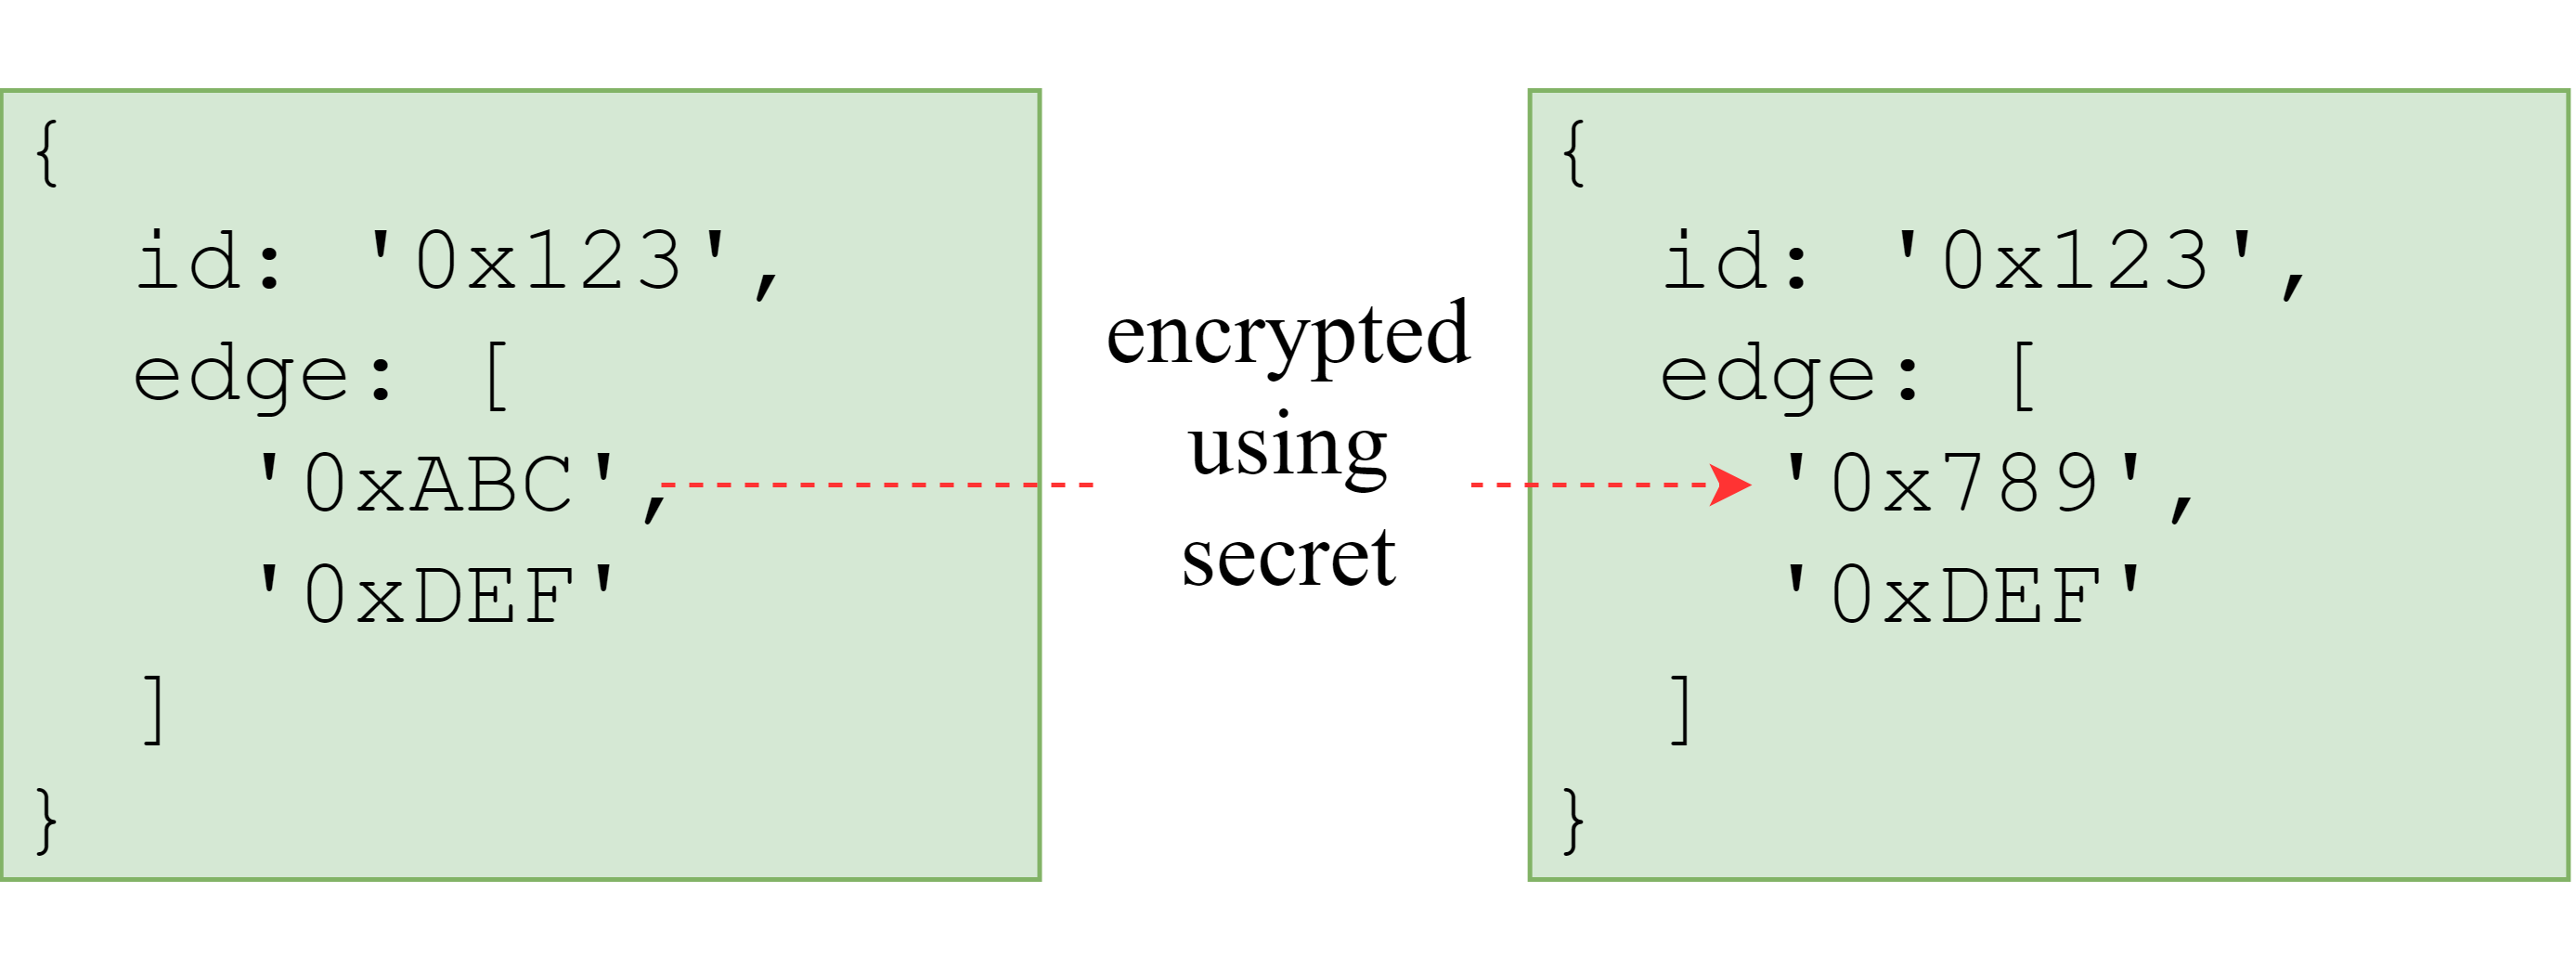
\includegraphics[height=1.02in]{data_for_privacy_example_as_tahoe_encrypted} %height = 17*.06
	\centering
	\caption{Event data in TAHOE format after encryption.}
	\label{fig:priv3}
\end{figure}

\subsubsection*{\textbf{Threat Model}}

The data owner \texttt{Org 2} does not trust anybody including CYBEX-P with the private attribute \texttt{1.1.1.1}.

\subsubsection*{\textbf{Private Data Query}}

\begin{figure}[ht]
	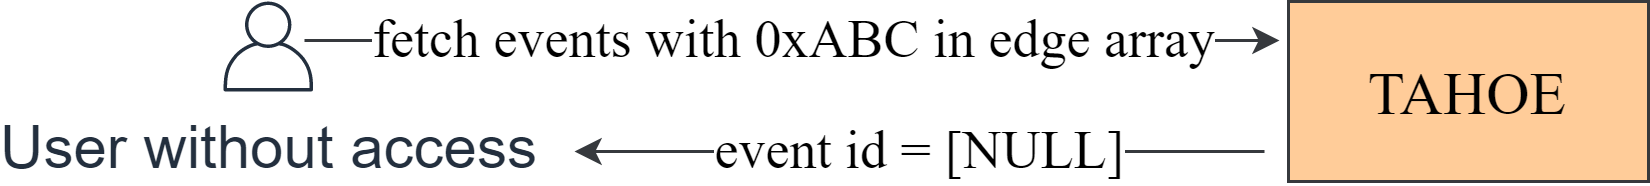
\includegraphics[height=.36in]{private_data_query} %height = 6*.06
	\centering
	\caption{Private Data Query.}
	\label{fig:privque}
\end{figure}

Now, a user wants to fetch all the \texttt{events} with the IP \texttt{1.1.1.1}. She first generates the hash of IP \texttt{1.1.1.1} as \texttt{0xABC}. Then she queries the database for \texttt{events} that have \texttt{0xABC} in their \texttt{edge} array. However, the database will return nothing, because the value \texttt{0xABC} is not present in any event edge. \texttt{Org 2} has essentially encrypted the graph edge.

\subsection{Private Attribute Sharing}

At this point, \texttt{Org 2} wants to share the private attribute \texttt{1.1.1.1} with \texttt{Org 3}. To achieve this, \texttt{Org 2} shares the \texttt{secret} with \texttt{Org 3}. CYBEX-P facilitates this sharing by providing a key management system (KMS) (\inlinefig{11} in Fig. \ref{fig:sysarch}).

\subsubsection*{\textbf{Threat Model}}

\texttt{Org 2} trusts \texttt{Org 3} and wants to share \texttt{1.1.1.1} with \texttt{Org 3}. However, \texttt{Org 2} does not trust CYBEX-P or any other user. \texttt{Org 2} shares the encryption \texttt{secret} with \texttt{Org 3} using CYBEX-P KMS.

\subsubsection*{\textbf{Private Data Query}}\label{sss:privq}

\begin{figure}[ht]
	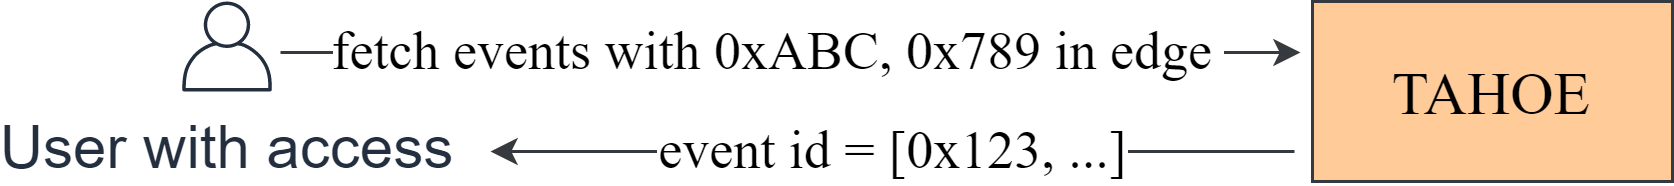
\includegraphics[height=.36in]{private_data_query_trusted} %height = 6*.06
	\centering
	\caption{Private Data Query by Trusted Party.}
	\label{fig:privquetrusted}
\end{figure}

Now, \texttt{Org 3} wants to fetch all \texttt{events} with the IP \texttt{1.1.1.1}. She first generates the hash of \texttt{1.1.1.1} as \texttt{0xABC}. Then she encrypts the hash with \texttt{secret} to generate the ciphertext \texttt{0x789}. Finally, she queries the database for \texttt{events} that have \texttt{0xABC} or \texttt{0x789} in the \texttt{edge} array. The database will return the \texttt{event 0x123} along with public events which include \texttt{1.1.1.1}. Note that, this query still makes one pass over the database.


\subsubsection*{\textbf{Private Data Correlation}}

A powerful feature of CYBEX-P is intrinsic correlation of data as described in \ref{ss:fcorr}. What makes TAHOE even more powerful is that, the intrinsic correlation mechanism works on encrypted data as well.

As explained in subsubsection \ref{sss:privq}, an authorized user can query encrypted data without revealing its value. The query performs a graph traversal, returning a complete graph of all the related \texttt{attributes} and \texttt{events}. This graph contains all the intrinsic correlations described in \ref{ss:fcorr}.

















\iffalse

\subsection{Revocation of Key}

Let's consider that after a while \texttt{Org 2} wants to stop sharing the private attribute \texttt{1.1.1.1} with \texttt{Org 3}. The only way to achieve a key revocation is the decrypt the private attribute and re-encrypt it using a new key.

\begin{figure}[ht]
	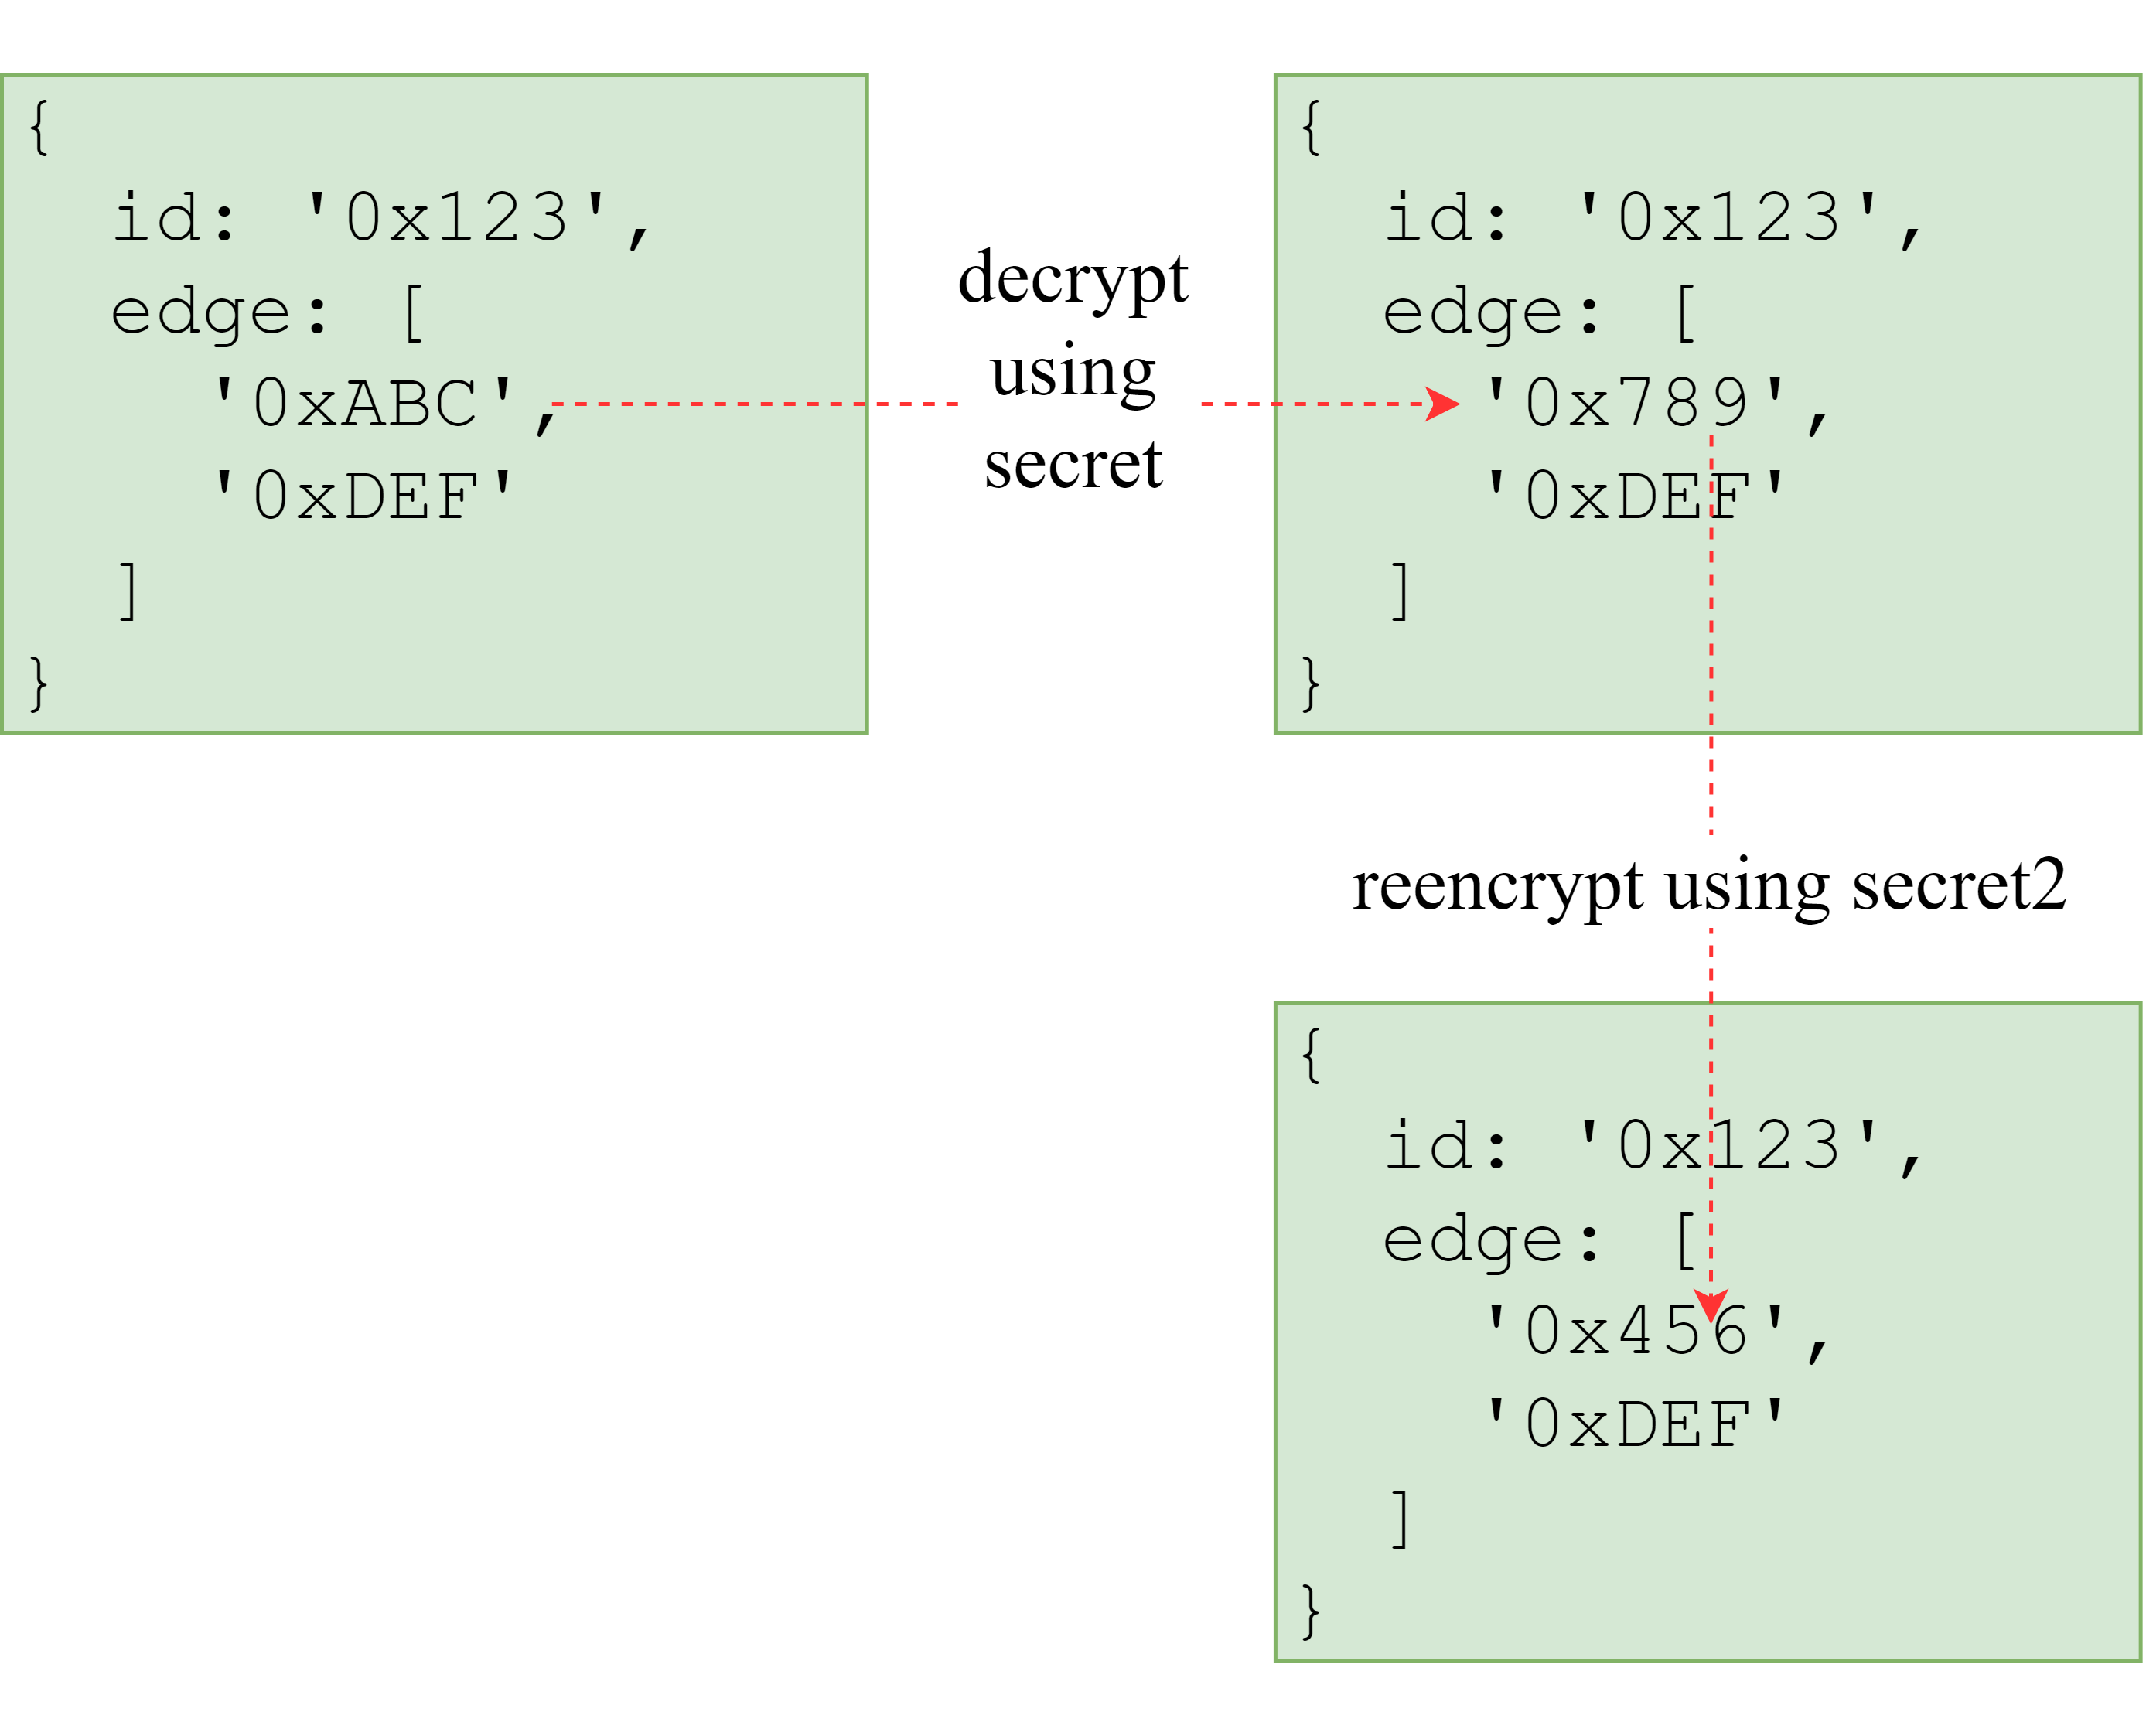
\includegraphics[width=\linewidth]{data_for_privacy_example_as_tahoe_revocation}
	\centering
	\caption{Revocation of key by re-encryption.}
	\label{fig:revocation}
\end{figure}

As shown in figure \ref{fig:revocation} \texttt{Org 2} decrypts the edge data using \texttt{secret} and re-encrypts the data using the new key \texttt{secret2}. This is will ensure that \texttt{Org 3} cannot access the data any longer.

\subsection{Secured Enclave with Intel SGX \& SCONE}

Our threat model considers CYBEX-P to be an untrusted entity. However, for the above data governance model to work CYBEX-P needs access to the uncrypted data or the plaintext in two cases: 1) CYBEX-P needs to analyse the plaintext to generate the hashes of the attribute 2) CYBEX-P needs to decrypt the data during revocation. A malicious actor with root access (e.g. admin of CYBEX-P) can potentially take a memory dump of the CYBEX-P server during these processes to get the plaintext data.

We take care of this issue by using a secured enclave to process the data. In this work we use Intel SGX \cite{costan2016intel} for attestation. We use SCONE \cite{199364} to interface with Intel SGX. SCONE is a configuration and attestation service (CAS) that uses Intel SGX. We use the SCONE platform execute part of our code inside a trusted execution environment. It can verify the integrity of the code and in turns ensure total privacy of user data. Following sections explain how we use SCONE.

\subsubsection{Application Audit}

Before sharing data, the data owner audits the source code in our SCONE installation. The data owner may choose any trusted person to audit the source code of our application along with the source code of our SCONE installation.

\begin{figure}[ht]
	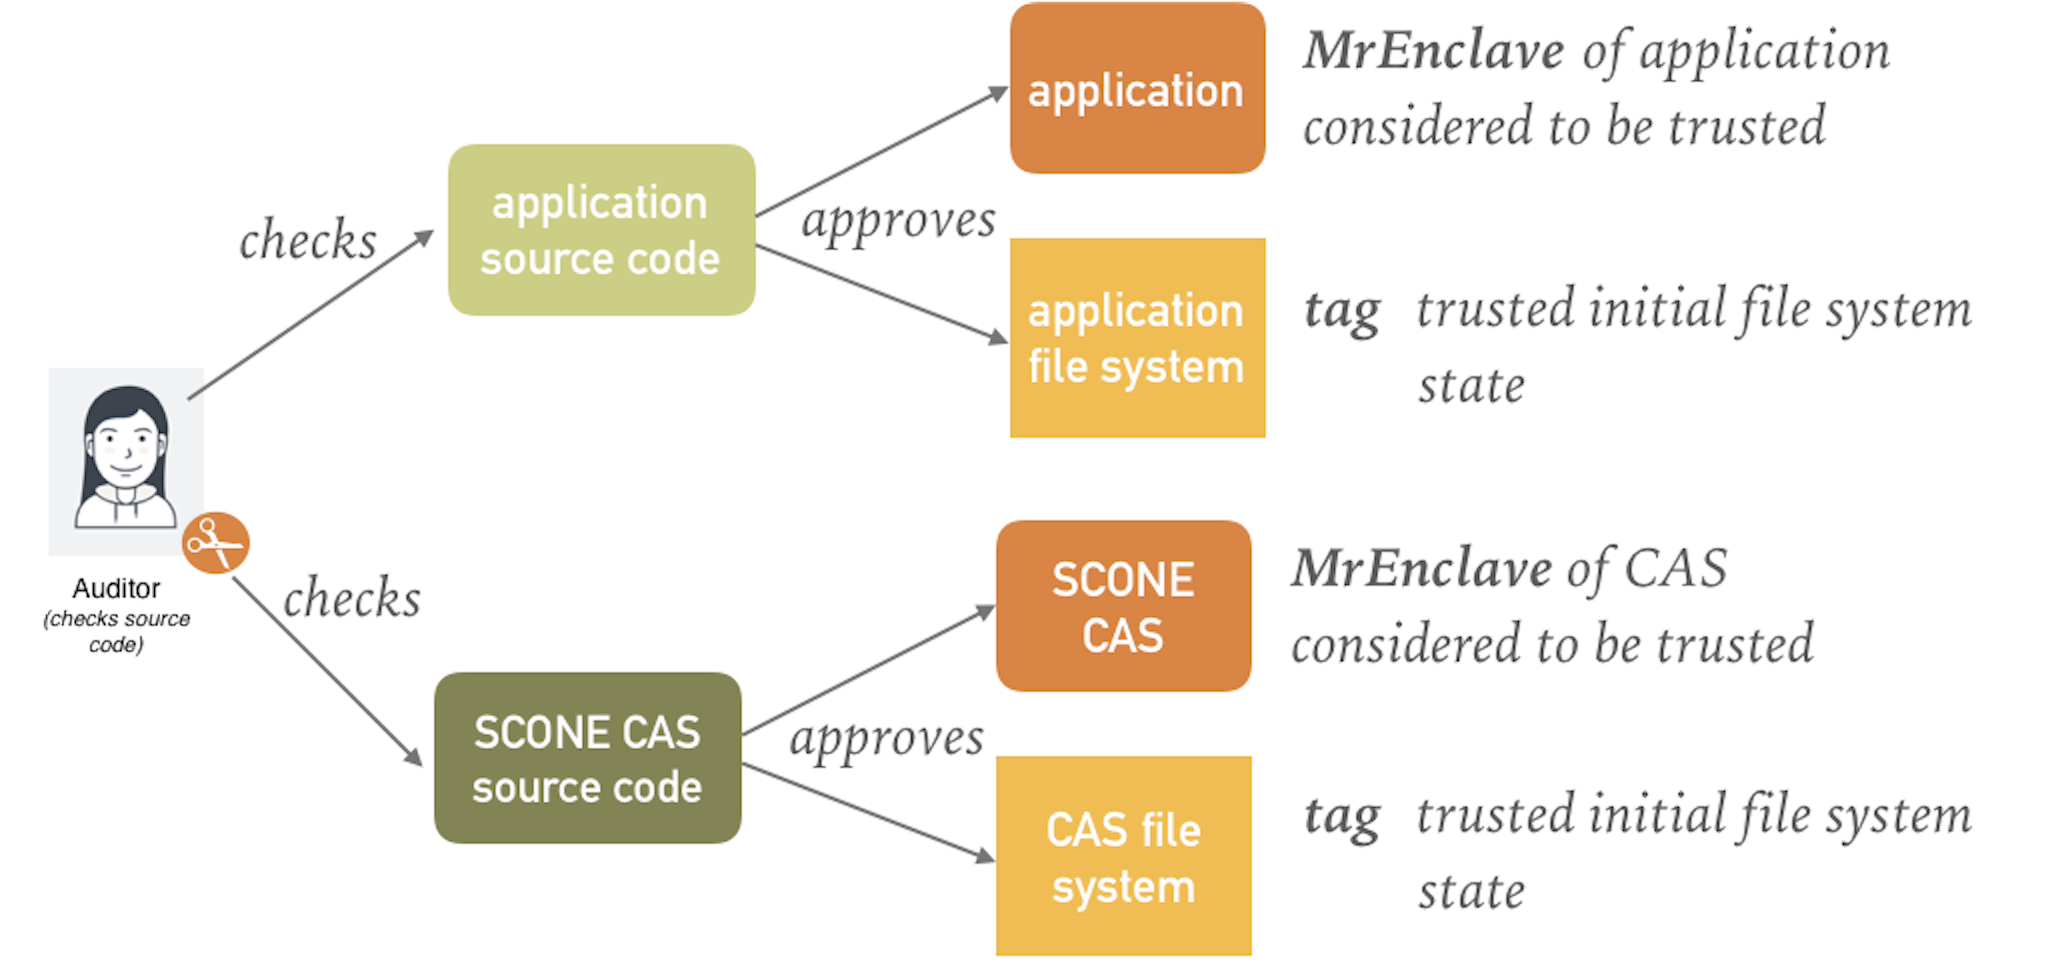
\includegraphics[width=\linewidth]{scone_auditor}
	\centering
	\caption{Auditor checks the application source code.}
	\label{fig:audit}
\end{figure}

The auditor first reads through the source code to verify that there are no loopholes or backdoors to access unencrypted data. We put only the necessary portion of our code in the SCONE subsystem, so that this step does not take a long time. Secondly, the auditor signs the enclave to generate a digest called a MrEnclave. Thirdly, the auditor determines the tags of the file system at that state. Any change in the file system would result in different tags. The auditor then does the same for the SCONE installation source code. After verifying bot the application and the SCONE installation the auditor shares the MrEnclave and the filesystem tags with the data owner.

This process while time consuming needs to be done only once. The ideal scenario in future is to get the code audited by a renown third party like the department of homeland security. In that case everyone in the industry can trust our system.

\subsubsection{User}

Once the code is audited and verified, the user shares his encrypted \texttt{secret} with the application. SCONE ensures that only the trusted application can access the decrypted \texttt{secret}. The user shares encrypted data with the secured enclave (for case 1 above) or requests CYBEX-P to share his data with the secured enclave (for case 2 above). Finally, the user instructs the verified application to perform the desired action.

\begin{figure}[ht]
	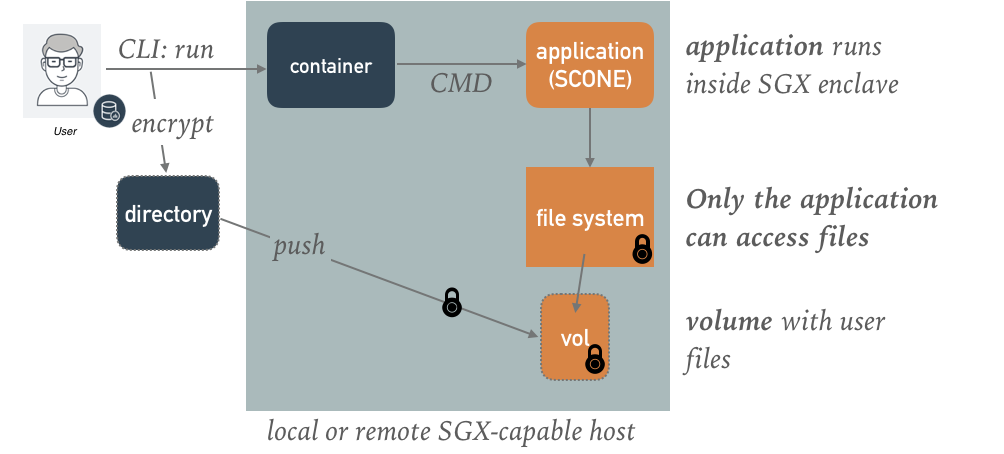
\includegraphics[width=\linewidth]{scone_user}
	\centering
	\caption{User shares the encrypted secret with the audited application.}
	\label{fig:user}
\end{figure}

\begin{figure}[ht]
	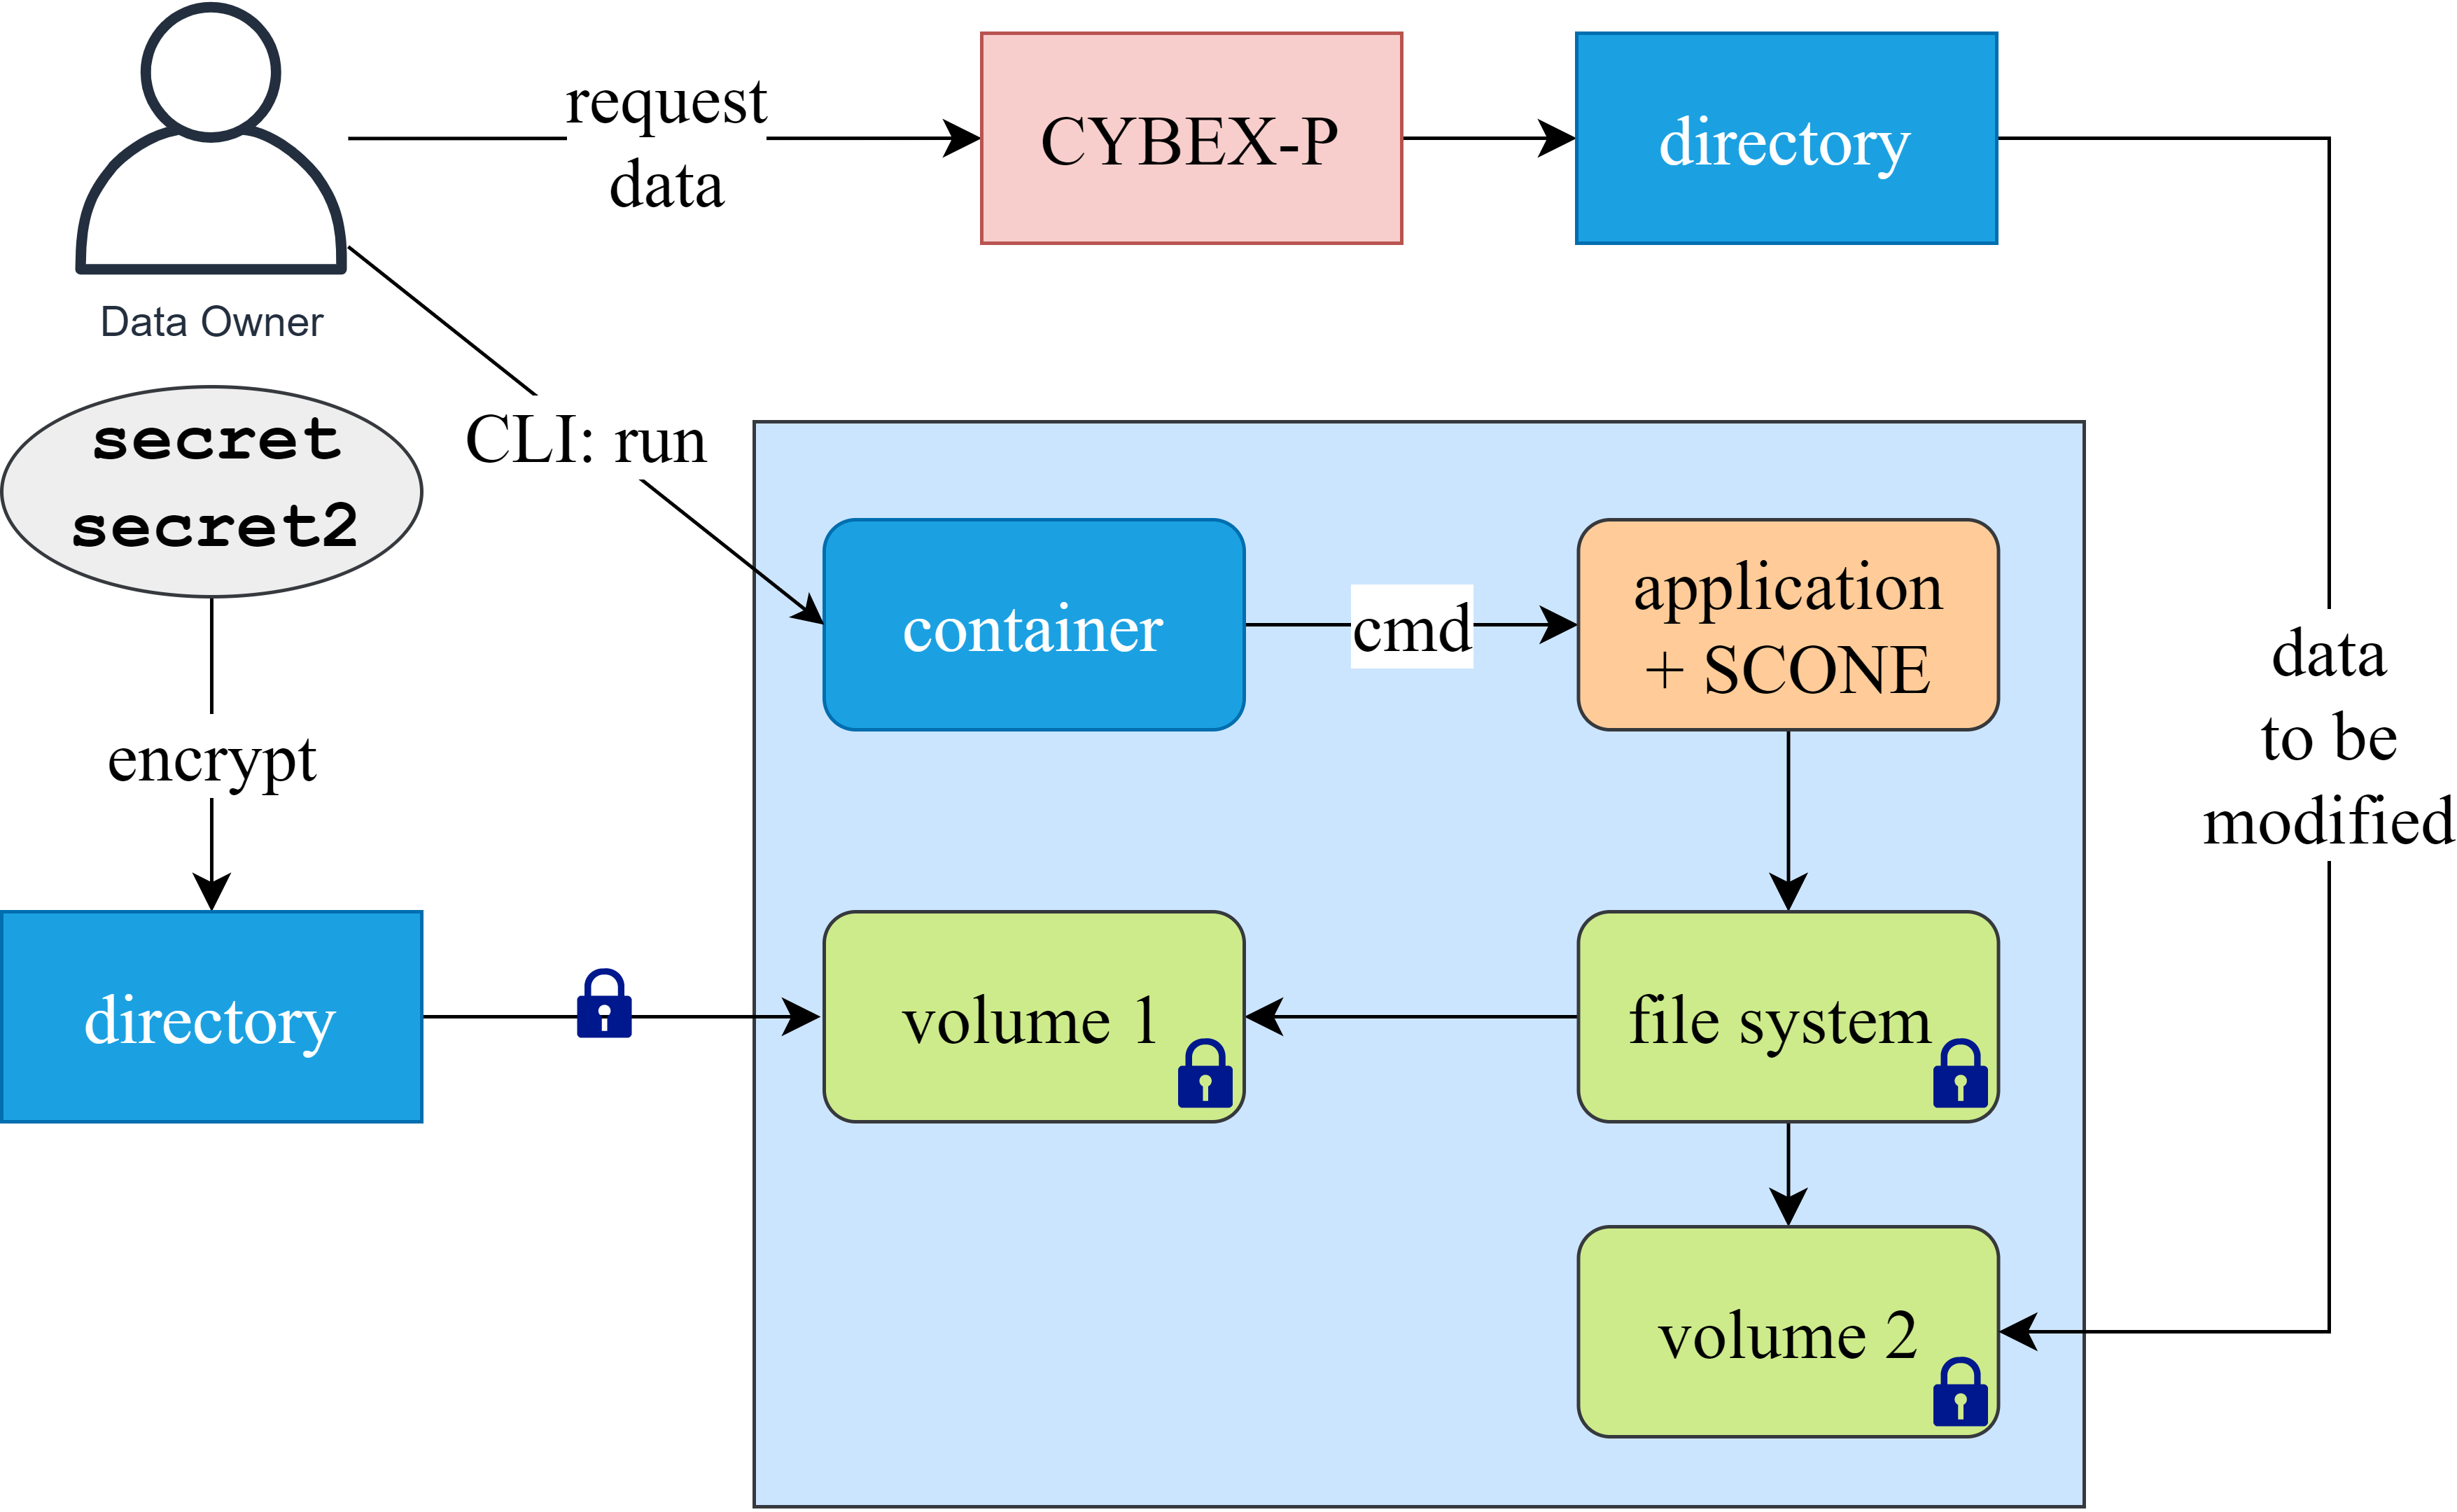
\includegraphics[width=\linewidth]{scone_revoke}
	\centering
	\caption{Key revocation using secured enclave.}
	\label{fig:revoke}
\end{figure}

The processing of data inside the enclave is trivial. There are two particular tasks that the user can perform in the secured enclave. The user can either parse his data into TAHOE format and encrypt the private edges. Or the user can decrypt certain edges and re-encrypt them using a new key to revoke the old key. The SCONE subsystem ensures that only the verified application can decrypt the data and/or the secrets.

\subsubsection{Attacker}

The attacker in this threat model is anybody who has root access to the CYBEX-P server. The data owner wants to limit such an attacker from accessing his data. Intel SGX achieves this by encrypting the data in use (in random access memory) and providing plaintext data to the CPU only. SCONE interfaces our code with Intel SGX.

\begin{figure}[ht]
	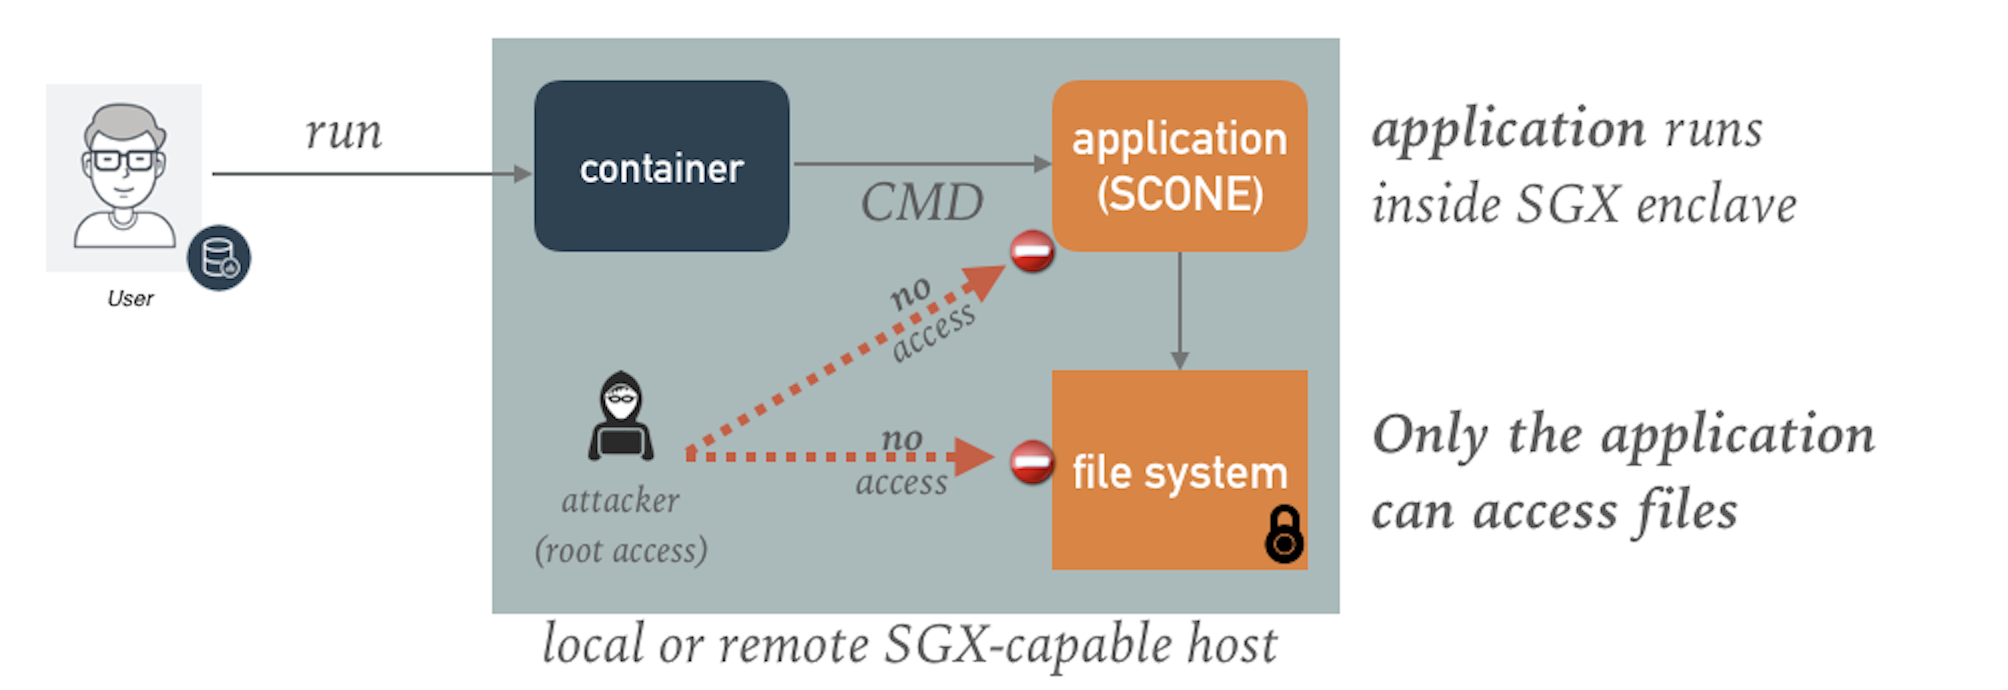
\includegraphics[width=\linewidth]{scone_attacker}
	\centering
	\caption{Root user cannot read encrypted RAM.}
	\label{fig:attacker}
\end{figure}

SCONE performs a transparent attestation of the application to ensure that neither the application nor the file system has been modified. Only then, SCONE transparently encrypts/decrypts the files. In this way, SCONE ensures the confidentiality and integrity of the data shared by the data owner.

\fi